
\documentclass{NUDTproposal}
%使用说明:
% 1. 开题报告的格式要求没那么严格,若提交没有格式异议则不用改。
% 2. 若需修改,可以直接在cls中做修改,或在github上提问题,关键是提供最新的word模板。
% 3. 字体若要更换,自行在cls文件中切换
% 4. 参考文献使用biblatex,需要用biber编译。
% 5. 图、表、公式,正常用figure,table,equation写即可。

%其他:
%添加想用的其他宏包,比如数学定理环境等等。
%设置参考文献数据库
\addbibresource{ref.bib}


\begin{document}

%设置论文信息
\NUDTvalueset
{
    author={谭同学},                % 作者
    title={这是一个很长的很长的学位论文题目这是一个很长的学位论文XXX大学开题报告\LaTeX{} 模板},                          % 论文标题
    schoollogo={
\includegraphics[scale=0.13]{nudt_logo_new}},
    schooltext={
\includegraphics[scale=0.35]{nudt_text_new}},
    proposaltype={\CJKunderline{博士}研究生学位论文}, % 研究生类别:硕士,博士需下划线
    classification={公开},          % 密级:公开,秘密,机密或者绝密
    proposalnumber={\underline{\makebox[1cm][c]{XXX}}},  % 编号:默认是下划线
    authorid={160590xx},            % 学号
    major={控制科学与工程},         % 一级学科
    field={图像处理},               % 研究方向
    advisor={张老师},               % 导师
    advisortitle={教~~~~授},        % 职称
    institute={信息系统与管理学院}, % 学院
    date={2017~年~03~月~01日},      % 开题日期
    mark={国防科技大学研究生院制},  % 制表单位信息
}

%绘制封面
\makecover


%正文内容
\zihao{5}

%各节可以在各个文件中给出,也可以直接在本文件中写。
%%%%% --------------------------------------------------------------------------------
%%
%%%%******************************* Main Content *************************************
%%
%%% ++++++++++++++++++++++++++++++++++++++++++++++++++++++++++++++++++++++++++++++++++


\section{学位论文选题的立论依据}

(课题来源、选题依据、理论与实际意义、预期研究成果的学术价值或应用价值等)

\subsection{课题来源}
自拟。


\subsection{基本概念}
\subsubsection{异常事件}
异常,新华词典的解释是“不同于平常”\upcite{Cong2011Sparse}。从分类的角度看,异常与正常是两个大类别,异常内部又可以分成打架、撞车等小类别。从概率的角度看\upcite{li2000},“平常”是大多数,而“异常”就是少数,所以异常事件,则可解释为“小概率事件”。
    异常事件的分类有很多角度。根据场景运动目标的多少,可以分为拥挤场景的异常事件和不拥挤场景的异常事件。这种分类主要根据基于跟踪和轨迹分析的异常检测方法能否适用。拥挤场景现有的跟踪方法都会失效,而不拥挤场景基于跟踪和轨迹分析的方法是可能奏效的。根据异常事件的规模,可以分为全局异常事件(如图 1)和局部异常事件(如图 2)。这种分类可以用于决定异常警报的级别。根据异常事件是基于先验知识还是场景学习,可以分为特定类型异常事件和广义异常事件\upcite{biber}。


\begin{figure}
    \centering
	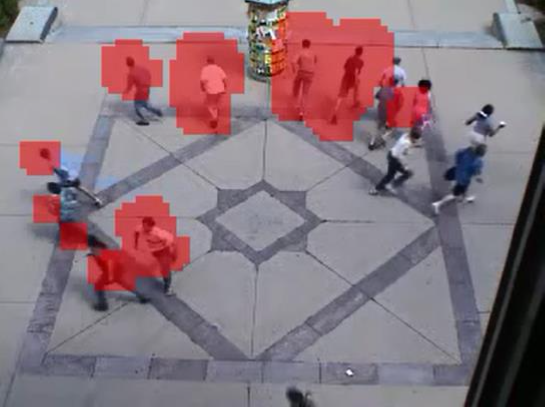
\includegraphics[width=0.7\linewidth]{fig1}
	\caption{人群四散逃离的异常事件(全局异常事件)}
	\label{fig:fig1}
\end{figure}

\begin{table}
    \centering
	\caption{一张表} \label{tab:tab1}
	\begin{tabular}{lrrr} \hline
		年份        & 乡村 & 城市 & 所有   \\ \hline
		1983        & 38.7  & 55.6  & 44.7  \\
		1993–1994   & 50.3  & 66.4  & 54.3  \\
		2004–2005   & 50.2  & 69.3  & 55    \\
		2009–2010   & 51.7  & 71.6  & 57.1  \\ \hline
		\multicolumn{4}{@{}l@{}}{\footnotesize 来源: http://tomheaven.cn}
	\end{tabular}
\end{table}

\begin{figure}
    \centering
	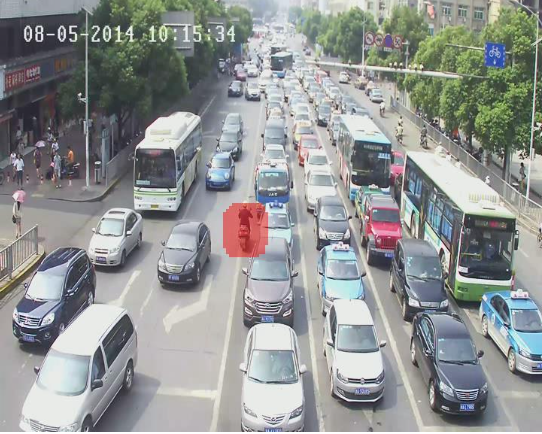
\includegraphics[width=0.7\linewidth]{fig2}
	\captionof{figure}{摩托车违章逆行的异常事件(局部异常事件)} % \caption{} 改为
	\label{fig:fig2}
\end{figure}




\subsubsection{广义异常事件}

本课题认为从分类的角度检测到的是特定类型异常事件,而从概率的角度检测到的是广义异常事件\upcite{li2000}。例如打架斗殴、人群逃散、交通事故都是根据人们的先验知识确定的异常事件,在绝大多数场景中,只要发生这样的事件,就肯定是异常事件。而广义异常事件与特定类型异常事件相对,是指不能由人们的先验知识预先设定类别,而是由监控视频场景决定的异常事件。发生概率低和与场景相关是广义异常事件的本质特征。

例如图 2的摩托车逆行,只有发生在此场景的城市道路上,才是异常事件。如果发生在了无人烟的乡村土路上并不算是异常。而摩托车是不是逆行,也只有放在此特定的场景中才能判断。

\subsection{研究意义}
    随着视频监控在商场、银行、小区、道路等公共场所的广泛部署\upcite{Cong2011Sparse},监控视频数据大量产生。目前监控视频主要还是用于威慑犯罪和事后调取,但视频智能分析的需要一直存在。近期发生了一些引起公众关注的事件再次体现了监控视频异常检测需求的迫切性。IBM深圳公司的一名女经理在地铁口突发心脏病跌倒,虽然正对着监控,却因为监控无人查看而耽误了抢救时间,最终不幸去世。对于这种紧急情况,仅有八分钟的黄金抢救时间,不能及时发现险情和施救生命就会逝去。
    监控视频的异常检测在安防领域、交通管理、城市管理方面有广阔的应用前景。从监控视频中自动发打架斗殴、交通违章、交通事故、人群聚集等事件具有及时发现事故险情,提前发现安全隐患的作用。例如图 3中的行人违规横穿马路,说明此路段存在交通安全隐患,有必要派出交警或者增设警示标志。如果这种情况持续发生,可以考虑架设人行天桥来引导行人。而这种安全隐患靠人工是很难发现和统计的。

  随着计算能力的不断进步,满足视频智能分析需求的计算成本在不断降低,视频智能分析的技术也在不断进步,为监控视频智能分析的普及准备着技术条件,智能监控的时代正在迫近。异常事件检测,作为视频智能分析的重要一环,能够帮助及早发现安全隐患,对异常事件实时发出警报,对于利用监控视频保障安全、处置险情,有重要作用\upcite{biblatex}。


%%% ++++++++++++++++++++++++++++++++++++++++++++++++++++++++++++++++++++++++++++++++++
%
\clearpage

%%%%% --------------------------------------------------------------------------------
%%
%%%%******************************* Main Content *************************************
%%
%%% ++++++++++++++++++++++++++++++++++++++++++++++++++++++++++++++++++++++++++++++++++


\section{文献综述}

(该选题在国内/外的研究现状及发展动态;阅读文献的范围以及查阅方式等。博士不得少于3000字,硕士不少于2000字。)

很多文献\upcite{yu2018spider}……



%%% ++++++++++++++++++++++++++++++++++++++++++++++++++++++++++++++++++++++++++++++++++
%
\clearpage

%%%%% --------------------------------------------------------------------------------
%%
%%%%******************************* Main Content *************************************
%%
%%% ++++++++++++++++++++++++++++++++++++++++++++++++++++++++++++++++++++++++++++++++++




\section{研究内容}

\subsection{研究目标}
1231231

\centerline{\rule[5pt]{\textwidth+2mm}{0.7pt}}% 表格中分割横线,勿删
\subsection{主要研究内容、需要解决的关键理论问题或技术问题}
123

\centerline{\rule[5pt]{\textwidth+2mm}{0.7pt}}% 表格中分割横线,勿删
\subsection{工作方案(研究方法、技术路线等)及可行性分析}

\subsubsection{公式}

公式正常写:
\begin{equation}\label{eq:eg:a}
  E=mc^2
\end{equation}

\centerline{\rule[5pt]{\textwidth+2mm}{0.7pt}}% 表格中分割横线,勿删
\subsection{预期创新点}

很多内容……



%%% ++++++++++++++++++++++++++++++++++++++++++++++++++++++++++++++++++++++++++++++++++
%
\clearpage

%%%%% --------------------------------------------------------------------------------
%%
%%%%******************************* Main Content *************************************
%%
%%% ++++++++++++++++++++++++++++++++++++++++++++++++++++++++++++++++++++++++++++++++++




\section{研究条件}


{\bfseries \kaishu \zihao{5} 开展研究应具备的条件及已具备的条件,可能遇到的困难与问题和解决措施。}


%%% ++++++++++++++++++++++++++++++++++++++++++++++++++++++++++++++++++++++++++++++++++
%
\clearpage

%%%%% --------------------------------------------------------------------------------
%%
%%%%******************************* Main Content *************************************
%%
%%% ++++++++++++++++++++++++++++++++++++++++++++++++++++++++++++++++++++++++++++++++++




\section{学位论文工作计划}
{
\noindent
\begin{tabular*}{0.999\textwidth}{| p{0.20\textwidth } <{\centering} | p{0.40\textwidth}  | p{0.311\textwidth}  |}

	\hline
	\multicolumn{1}{|c|}{起讫日期} & 	\multicolumn{1}{c}{主要完成研究内容} & 	\multicolumn{1}{|c|}{预期成果} \\
	\hline
	\makecell{2017年09月 -- \\2018年03月}   &  基础知识学习 &   完成文献搜集与该方向基本知识储备 \\
	\hline
	\makecell{2018年04月 -- \\2018年06月} &  研究点1 &   完成实验 \\
	\hline
	\makecell{2018年07月 -- \\2018年08月} &  研究点1 &   发表论文SCI一篇 \\
	\hline
	\makecell{2018年09月 -- \\2018年10月} &  研究点2 &   完成实验 \\
	\hline
    \makecell{2018年11月 -- \\2018年12月} &  研究点2 &   发表论文EI一篇 \\
    \hline
    \makecell{2019年01月 -- \\2019年02月} &  研究点3 &   完成实验 \\
    \hline
    \makecell{2019年03月 -- \\2019年04月} &  研究点3 &   发表论文EI一篇 \\
    \hline
    \makecell{2019年05月 -- \\2019年06月} &  研究点4 &   完成实验 \\
    \hline
    \makecell{2019年07月 -- \\2019年08月} &  研究点4 &   发表论文EI一篇 \\
    \hline
    \makecell{2019年09月 -- \\2019年09月} &  研究点5 &   完成实验 \\
    \hline
    \makecell{2019年10月 -- \\2019年10月} &  研究点5 &   发表论文EI一篇 \\
    \hline
	\makecell{2019年11月 -- \\2020年01月} &  撰写毕业论文 &  完成毕业论文 \\
	\hline
\end{tabular*}
\\[1 cm]
{\songti 注:每个子阶段不得超过3个月;预期成果中必须包含成果的形式、数量、质量等可考性指标该计划将作为
论文研究进展检查的依据。}
\indent
}


%%% ++++++++++++++++++++++++++++++++++++++++++++++++++++++++++++++++++++++++++++++++++
%
\clearpage


%参考文献使用biblatex,用biber编译
%参考文献的表格若行高不够,则利用命令\setlength\tabrowheight{1cm}设置更大的行高
\section{主要参考文献}
{\renewcommand{\bibfont}{\footnotesize}
\printbibtabular[heading=none]
}
\clearpage


%导师评价,可以先签字后替换或者利用电子签名
%%%%% --------------------------------------------------------------------------------
%%
%%%%******************************* Main Content *************************************
%%
%%% ++++++++++++++++++++++++++++++++++++++++++++++++++++++++++++++++++++++++++++++++++




\section{指导教师对开题报告的评语}
\indent {\songti{(对1-6项逐项予以评价,并着重对国内/外研究现状的了解情况、研究内容的创新性等方面进行评价,
最终给出是否满足博士/硕士层次学位论文研究要求的综合评价意见)}}

课题评价。……

符合博士研究生开题要求。


\begin{flushright}
    \songti{导师签字:}\ \ \ \ \ \ \ \ \ \ \ \ \ \ \ \ \ \ \ \ \ \ \ \ \ \ \ \ \ \
    \vspace{10 mm}

    \ \ \ \ \ \ \ \ \ \ \ 年 \ \ \ \ \ \ 月 \ \ \ \ \ \ \ 日
    \vspace{30 mm}
\end{flushright}


%%% ++++++++++++++++++++++++++++++++++++++++++++++++++++++++++++++++++++++++++++++++++
%
\clearpage

%评审意见直接插进来就行,最终版用签字扫描版替代
\includepdf[pages=-]{研究生学位论文开题报告评议表.pdf}
\clearpage




\end{document} 